\documentclass[a4,useAMS,usenatbib,usegraphicx]{latex/mn2e} 
%\documentclass{latex/emulateapj} 
%External Packages and personalized macros
%=========================================================================
%		EXTERNAL PACKAGES
%=========================================================================
\usepackage{amsmath} 
\usepackage{amssymb} 
\usepackage[section]{placeins}
\usepackage {graphicx}
%\usepackage{graphics}
\usepackage[dvips]{epsfig}
\usepackage{epsfig}  
\usepackage{color}
\usepackage[normalem]{ulem}
\usepackage{hyperref}
\usepackage{caption}
%Non reposionated tables
\usepackage{float}
\restylefloat{table}

%=========================================================================
%		INTERNAL MACROS
%=========================================================================
\def\be{\begin{equation}}
\def\ee{\end{equation}}
\def\ba{\begin{eqnarray}}
\def\ea{\end{eqnarray}}

% To highlight comments 
\definecolor{red}{rgb}{1,0.0,0.0}
\newcommand{\red}{\color{red}}
\definecolor{darkgreen}{rgb}{0.0,0.5,0.0}
\newcommand{\SRK}[1]{\textcolor{darkgreen}{\bf SRK: \textit{#1}}}
\newcommand{\SRKED}[1]{\textcolor{darkgreen}{\bf #1}}

\newcommand{\LCDM}{$\Lambda$CDM~}
\newcommand{\beq}{\begin{eqnarray}}  
\newcommand{\eeq}{\end{eqnarray}}  
\newcommand{\zz}{$z\sim 3$} 
\newcommand{\apj}{ApJ}  
\newcommand{\apjs}{ApJS}  
\newcommand{\apjl}{ApJL}  
\newcommand{\aj}{AJ}  
\newcommand{\mnras}{MNRAS}  
\newcommand{\mnrassub}{MNRAS accepted}  
\newcommand{\aap}{A\&A}  
\newcommand{\aaps}{A\&AS}  
\newcommand{\araa}{ARA\&A}  
\newcommand{\nat}{Nature}  
\newcommand{\physrep}{PhR}
\newcommand{\pasp}{PASP}    
\newcommand{\pasj}{PASJ}    
\newcommand{\avg}[1]{\langle{#1}\rangle}  
\newcommand{\ly}{{\ifmmode{{\rm Ly}\alpha}\else{Ly$\alpha$}\fi}}
\newcommand{\hMpc}{{\ifmmode{h^{-1}{\rm Mpc}}\else{$h^{-1}$Mpc }\fi}}  
\newcommand{\hGpc}{{\ifmmode{h^{-1}{\rm Gpc}}\else{$h^{-1}$Gpc }\fi}}  
\newcommand{\hmpc}{{\ifmmode{h^{-1}{\rm Mpc}}\else{$h^{-1}$Mpc }\fi}}  
\newcommand{\hkpc}{{\ifmmode{h^{-1}{\rm kpc}}\else{$h^{-1}$kpc }\fi}}  
\newcommand{\hMsun}{{\ifmmode{h^{-1}{\rm {M_{\odot}}}}\else{$h^{-1}{\rm{M_{\odot}}}$}\fi}}  
\newcommand{\hmsun}{{\ifmmode{h^{-1}{\rm {M_{\odot}}}}\else{$h^{-1}{\rm{M_{\odot}}}$}\fi}}  
\newcommand{\Msun}{{\ifmmode{{\rm {M_{\odot}}}}\else{${\rm{M_{\odot}}}$}\fi}}  
\newcommand{\msun}{{\ifmmode{{\rm {M_{\odot}}}}\else{${\rm{M_{\odot}}}$}\fi}}  
\newcommand{\lya}{{Lyman$\alpha$~}}
\newcommand{\clara}{{\texttt{CLARA}}~}
\newcommand{\rand}{{\ifmmode{{\mathcal{R}}}\else{${\mathcal{R}}$ }\fi}}  
%SAMPLES
\newcommand{\GHBDM}{\texttt{GH}$_{\mbox{\tiny{BDM}}}$ }
\newcommand{\GHFOF}{\texttt{GH}$_{\mbox{\tiny{FOF}}}$ }
\newcommand{\IHBDM}{\texttt{IH}$_{\mbox{\tiny{BDM}}}$ }
\newcommand{\IHFOF}{\texttt{IH}$_{\mbox{\tiny{FOF}}}$ }
\newcommand{\PBDM}{\texttt{P}$_{\mbox{\tiny{BDM}}}$ }
\newcommand{\PFOF}{\texttt{P}$_{\mbox{\tiny{FOF}}}$ }
\newcommand{\IPBDM}{\texttt{IP}$_{\mbox{\tiny{BDM}}}$ }
\newcommand{\IPFOF}{\texttt{IP}$_{\mbox{\tiny{FOF}}}$ }
\newcommand{\RIPBDM}{\texttt{RIP}$_{\mbox{\tiny{BDM}}}$ }
\newcommand{\RIPFOF}{\texttt{RIP}$_{\mbox{\tiny{FOF}}}$ }


%MY COMMANDS #############################################################
\newcommand{\sub}[1]{\mbox{\scriptsize{#1}}}
\newcommand{\dtot}[2]{ \frac{ d #1 }{d #2} }
\newcommand{\dpar}[2]{ \frac{ \partial #1 }{\partial #2} }
\newcommand{\pr}[1]{ \left( #1 \right) }
\newcommand{\corc}[1]{ \left[ #1 \right] }
\newcommand{\lla}[1]{ \left\{ #1 \right\} }
\newcommand{\bds}[1]{\boldsymbol{ #1 }}
\newcommand{\oiint}{\displaystyle\bigcirc\!\!\!\!\!\!\!\!\int\!\!\!\!\!\int}
\newcommand{\mathsize}[2]{\mbox{\fontsize{#1}{#1}\selectfont $#2$}}
\newcommand{\eq}[2]{\begin{equation} \label{eq:#1} #2 \end{equation}}
\newcommand{\lth}{$\lambda_{th}$ }
%#########################################################################

\begin{document}

%=========================================================================
%		FRONT MATTER
%=========================================================================
\title{Tidal field anisotropy as a tracer of cosmic voids}
\author[S. Bustamante and J.E. Forero-Romero]{
\parbox[t]{\textwidth}{\raggedright 
  Sebastian Bustamante \thanks{sebastian.bustamante@udea.edu.co}$^{1}$,
  Jaime E. Forero-Romero$^{2}$ 
}
\vspace*{6pt}\\
$^1$Instituto de F\'{\i}sica - FCEN, Universidad de Antioquia, Calle
67 No. 53-108, Medell\'{\i}n, Colombia\\ 
$^2$Departamento de F\'{i}sica, Universidad de los Andes, Cra. 1
No. 18A-10, Edificio Ip, Bogot\'a, Colombia
}

\maketitle

\begin{abstract}
Finding and characterizing underdense regions (voids) in the large
scale structure of the Universe is an important task in cosmological
studies.  
In this paper we present a novel approach to find voids in
cosmological simulations.  
Our approach is based on algorithms that use the tidal and the
velocity shear tensors to locally define the cosmic web.
Voids are identified using the fractional anisotropy (FA) computed
from the eigenvalues of each web scheme. 
We define the void boundaries using a watershed transform based on the
local minima of the FA and its boundaries as the regions where the FA
is maximized
This void identification technique does not have any free parameters
and does not make any assumption on the shape or structure of the
voids.  
We test the method on the Bolshoi simulation and report on the density
and velo ity profiles for the voids found using this new scheme. 
\end{abstract}

\begin{keywords}
Cosmology: theory - large-scale structure of Universe -
Methods: data analysis - numerical - N-body simulations
\end{keywords}


%=========================================================================
%		PAPER CONTENT
%=========================================================================

%*************************************************************************
\section{Introduction}
\label{sec:introduction}
%*************************************************************************


Since voids were found in the first compiled galaxy surveys 
they have been identified as one of the most striking features of the
Cosmic Web \citep{Chincarini75,  Gregory78, Einasto80M, Einasto80N,
  Kirshner81, Zeldovich82,Kirshner87, Bond96}. 
However,  due to the large volume extension of void regions ($\sim
5-10\ \mbox{Mpc}  h^{-1}$), statistically meaningful catalogues of
voids \citep{Pan10,  Sutter12b, Nadathur14} have only become available
through  modern galaxy surveys like the two-degree field Galaxy
Redshift Survey \citep{ Colless01, Colless03} and the Sloan Digital
Sky Survey \citep{York00, Abazajian03}.
This advancement generated a great interest to study voids
observationally during the last decade \citep{Hoyle04, Croton04, Rojas05,
  Ceccarelli06, Patiri06a, Tikhonov06, Patiri06b,Tikhonov07,
  BendaBeckmann08, Foster09, Ceccarelli13, Sutter14a}. 


On the theoretical side the rough theoretical framework that explains
the origin of voids was established in the seminal work of
\citet{Zeldovich70} and refined in the following decades.  
The first detailed theoretical models describing formation, dynamics
and properties of  voids \citep{Hoffman82, Icke84, Bertschinger85,
  Blumenthal92} were  complemented and extended by numerical studies
\citep{Martel90, Regos91, Weygaert93, Dubinski93, Bond96}. 
Currently, the dominant tendency to study voids relies on using data
from N-body simulations. For an extensive compilation of previous 
numerical works we refer the reader to \citet{Colberg08}.


The relevance of voids to cosmological studies can be summarized in
three aspects \citep{Platen07}. 
First, voids are a key ingredient of the Cosmic Web. 
They dominate the volume distribution at large-scales and
additionally, they compensate overdense structures in the total budget
of  matter.  
Second, voids provide a valuable resource for inferring and probing 
cosmological parameters as their structure and dynamics are highly 
determined by these values. 
Third, they are a  largely a largely pristine environment to test
galaxy evolution.


Although a visual recognition of voids in galaxy surveys and simulations
is possible in most cases, a formal systematic identification is desirable
for statistical studies. 
However, the community does not have an unambiguous definition of cosmic
voids. 
There are nany different void finding techniques in the literature
(for a detailed comparison of different schemes,  see the Void Finder
Comparison Project \citet{Colberg08}). 
In spite of the diversity of existing schemes, they can be roughly
classified into two main types. First, geometric schemes based on
point spatial or redshift  distribution of galaxies in surveys or dark
matter halos in  simulations \citep{Kauffmann91, Muller00,
  Gottlober03, Hoyle04, Brunino07,  Foster09, Micheletti14, Sutter14};
second, schemes based on the smooth  and continuous matter density
field either from simulations or from  reconstruction procedures on
surveys \citep{Plionis02, Colberg05,  Shandarin06, Platen07,
  Neyrinck08, MunozCuartas11, Neyrinck13, Ricciardelli2013}.


Here we introduce a new tracer of the structure of cosmic voids that
can be used once the continous matter density or velocity distribution
is known. 
The algorithm is based on two tensorial schemes used to classify the
cosmic web. 
The first (the T-web) is based on the Hessian of the gravitational potential or
tidal tensor \citep{Hahn07, Forero09}. 
The second (the V-web) is based on the velocity shear tensor
\citep{Hoffman12}. 
These web schemes classify the Cosmic Web into four different types of
environment depending on the counting of the number of eigenvalues below an 
user-defined threshold ($\lambda_{rm th}$): voids, sheets, filaments and
knots for $3,2,1$ or $0$ eigenvalues below $\lambda_{\rm th}$, respectively.

This procedure allows a new description of the internal structure
of voids that goes beyond a simple definition of a void as just an
underdense regions in the large-scale matter distribution.
The tidal and the shear tensors encode more information than the
density field as they trace the collapsing or expanding
nature of the matter field, which defines the dynamics of the Cosmic
Web. 

The tracer that we use to define the voids is the fractional
anisotropy (FA) computed from the set of eigenvalues of the tensor
under consideration. 
The FA was initially introduced by \citet{Basser95} to quantify the
anisotropy degree of the diffusivity of water molecules through
cerebral tissue in nuclear magnetic resonance
imaging.
\citet{Libeskind13} introduced this concept in the context of Cosmic
Web classification schemes.

Once we establish the FA as a void tracer, we proceed to
identify individual voids as basins of local minima. 
For this we implement a \textit{watershed transform algorithm}
\citep{Beucher79,Beucher93} which has been used to define as catching
basins of local minima of the density field
\citep{Platen07,Neyrinck08}; we use insted minima of the FA field to
find define the voids. 


This paper is organized as follows. 
In Section \ref{sec:algorithms_cosmic_web} we describe the algorithms
we use to find the cosmic web in N-body simulations. In Section 
\ref{sec:simulations} we describe the used simulation.
Then in Section \ref{sec:bulk_voids} we explain in detail our void
finder based on the fractional anisotropy of the tidal and shear
tensor fields.
%In Section \ref{sec:experiments} we describe the numerical experiments
%we perform to show the performance of the new void finding technique.
Our results are presented in \ref{sec:results} to finally comment and
conclude about these findings in Section \ref{sec:conclusions}. 


%*************************************************************************
\section{Algorithms to label the Cosmic Web}
\label{sec:algorithms_cosmic_web}
%*************************************************************************


%-------------------------------------------------------------------------
\subsection{The tidal web (Tweb)}
\label{subsec:Tweb}
%-------------------------------------------------------------------------


This scheme was initially proposed by \citet{Hahn07} as an
alternative for classifying the Cosmic Web based on the tidal tensor.
The tidal tensor allows a classification in terms of the orbital
dinamics of the matter field
This approach extends to second-order the equations of motion around 
local minima of the gravitational potential. 
The second-order term corresponds to the tidal tensor, which is
defined as the Hessian matrix of the normalized gravitational
potential.


%.........................................................................
%Tidal Tensor
\eq{V_web}
{	T_{\alpha\beta} = \frac{\partial^2\phi}{\partial x_{\alpha}\partial x_{\beta}},	}
%.........................................................................
where the physical gravitational potential has been rescaled by a
factor of   $4\pi G\bar{\rho}$ in such a way that $\phi$ satisfies the following 
Poisson equation

%.........................................................................
%Poisson
\eq{Poisson}
{	\nabla^2\phi = \delta,	}
%.........................................................................
with $\bar{\rho}$ the average density in the Universe, $G$ the 
gravitational constant and $\delta$ the dimensionless matter
overdensity. 


Since the tidal tensor can be represented by a real and  symmetric
$3\times 3$ matrix, it is always possible to diagonalize  
it and obtain three real eigenvalues $\lambda_{1}\geq\lambda_{2}\geq
\lambda_3$ with its corresponding eigenvectors ${\bf u}_{1}$, ${\bf u}_{2}$,
${\bf u}_{3}$. 
This set of eigenvalues are indicators of the local  orbital stability
in each direction ${\bf u}_i$, which is to label the Cosmic Web.
The number of positive (stable) or negative (unstable) eigenvalues allows 
to label a location into one of the next four types of environment: 
voids (3 negatives eigenvalues), sheets (2), filaments (1) and knots (0). 
A modification to this scheme was introduced by \citet{Forero09}
by means of a relaxation of the stability criterion. The relative strength 
of each eigenvalue is no longer defined by the sign, but instead by a
threshold value $\lambda_{\rm th}$ that can be tuned in such a way
that the visual impression of the web-like matter distribution is
reproduced. 
 
%-------------------------------------------------------------------------
\subsection{The velocity web (Vweb)}
\label{subsec:Vweb}
%-------------------------------------------------------------------------


We also use a kinematic scheme to define the Cosmic Web environment in 
the simulation, which has been thoroughly described in 
\cite{Hoffman12}.
This scheme has been used to study the shape, spin and peculiar
velocity alignments of dark matter halos with the cosmic web
\citep{Libeskind13,Forero2014}. 
We refer the reader to these papers to find a detailed description of
the algorithm, its limitations  and capabilities.    
The Vweb scheme for environment finding is based on the
local velocity shear tensor calculated from the smoothed dark matter 
velocity field in the simulation. This tensor is given by the 
following expression

%.........................................................................
%V-Web Definition
\eq{V_web}
{	\Sigma_{\alpha\beta} = -\frac{1}{2H_0}\pr{\frac{\partial v_{\alpha}}
{\partial x_{\beta}}+\frac{\partial v_{\beta}}{\partial x_{\alpha}}},}
%.........................................................................
where $v_{\alpha}$ and $x_{\alpha}$ represent the $\alpha$ component of 
the comoving velocity and position, respectively. Like the tidal tensor, 
$\Sigma_{\alpha\beta}$ can be represented by a $3\times 3$ symmetric 
matrix with real values, making it possible to find three real
eigenvalues and its corresponding eigenvectors.
%$\lambda_{1}\geq\lambda_{2}\geq\lambda_3$.
%whose sum (the 
%trace of $\Sigma_{\alpha\beta}$) is proportional to the divergence of the 
%local velocity field smoothed on the physical scale ${\mathcal R}$. 

In this case we also use the relative strength of the three eigenvalues with 
respect to a threshold value $\lambda_{th}$ to classify the cosmic web
in the four web types we have already described.

Usually, the threshold is a free parameter that is tuned to reproduce
the visual appearence of the comic web. 
In this paper we take a different approach.
We find the optimal value of the threshold based on the maximization
of the fractional anisotropy field in the locations label as filaments
and walls. 


\section{Numerical Simulations}
\label{sec:simulations}

We use the Bolshoi simulation to test the method describe in the
paper. 
This simulation follows the non-linear evolution of a dark
matter density field on a cubic volume of  size $250$\hMpc\ sampled
with $2048^3$ particles. 
The cosmological parameters in the simulation are $\Omega_{\rm m}=0.27$,  $\Omega_{\Lambda}  =0.73$, $h=0.70$,
$n=0.95$ and $\sigma_{8}=0.82$ for the matter density,   cosmological
constant, dimensionless Hubble parameter, spectral index of
primordial density perturbations and normalization for the power
spectrum, respectively. 
This values are consistent with the seventh year of data of the Wilkinson 
Microwave Anisotropy Probe (WMAP) \citep{Jarosik11}. 
For more detailed  technical information about the simulation, see
\citet{Klypin11}. 


We find the cosmic web we estimate first the density and velocity
fields using a  \textit{cloud-in-cell} (\texttt{CIC}) algorithm onto a grid of $256^3$ 
cells, corresponding to a spatial resolution of $0.98$\hMpc\ per cell
side.  
These fields are smoothed with a gaussian filter with a width of
$\sigma=0.98$\hMpc.
We compute the tidal and shear tensors through finite-differences and
Finally, the eigenvalues and eigenvectors of the tensor are
obtained for each grid cell.
The data we use here is publicly available through the MultiDark
database \url{http://www.multidark.org/MultiDark/} which is described
in \citet{Riebe11}.



%*************************************************************************
\section{A new void finding technique}
\label{sec:bulk_voids}
%*************************************************************************


%-------------------------------------------------------------------------
\subsection{The fractional anisotropy}
\label{subsec:FA_voids}
%-------------------------------------------------------------------------


The fractional anisotropy (FA), as developed by \citet{Basser95}, was 
conceived to quantify the anisotropy degree of a diffusion process, e.g. 
the diffusivity of water molecules through cerebral tissue in nuclear
magnetic resonance imaging. 
Here we propose the FA, much in the same way as \citet{Libeskind13},
as a tracer of cosmic voids. 


The FA is defined as follows.
%.........................................................................
%Fractional anisotropy
\eq{fractional_anisotropy}
{{\mathrm{FA}} = \frac{1}{\sqrt{3}}\sqrt{ \frac{ (\lambda_1 - \lambda_3)^2 + 
(\lambda_2 - \lambda_3)^2 + (\lambda_1 - \lambda_2)^2}{ \lambda_1^2 + 
\lambda_2^2 + \lambda_3^2} },}
%.........................................................................
where the eigenvalues are taken from either the Tweb or the Vweb 
(FA-Tweb and FA-Vweb respectively). Such as it is defined, FA$=0$ 
corresponds to an isotropic distribution ($\lambda_1=\lambda_2=\lambda_3$) 
and FA$=1$ with a highly anisotropic distribution.


In left panels of Fig. \ref{fig:FA_field} we show the FA field for both 
web schemes over a slide of the simulation. 
From this Figure we can observe that both, voids and knots, display a highly 
isotropic expanding dynamic at their centres, becoming gradually more
anisotropic at outer regions. 
On the other hand the filamentary structure is traced by high FA
values. These characteristics are the key to use the FA as a tracer of
cosmic voids. 

%.........................................................................
%FIGURE 1: FA and vissual impression
\begin{figure*}
  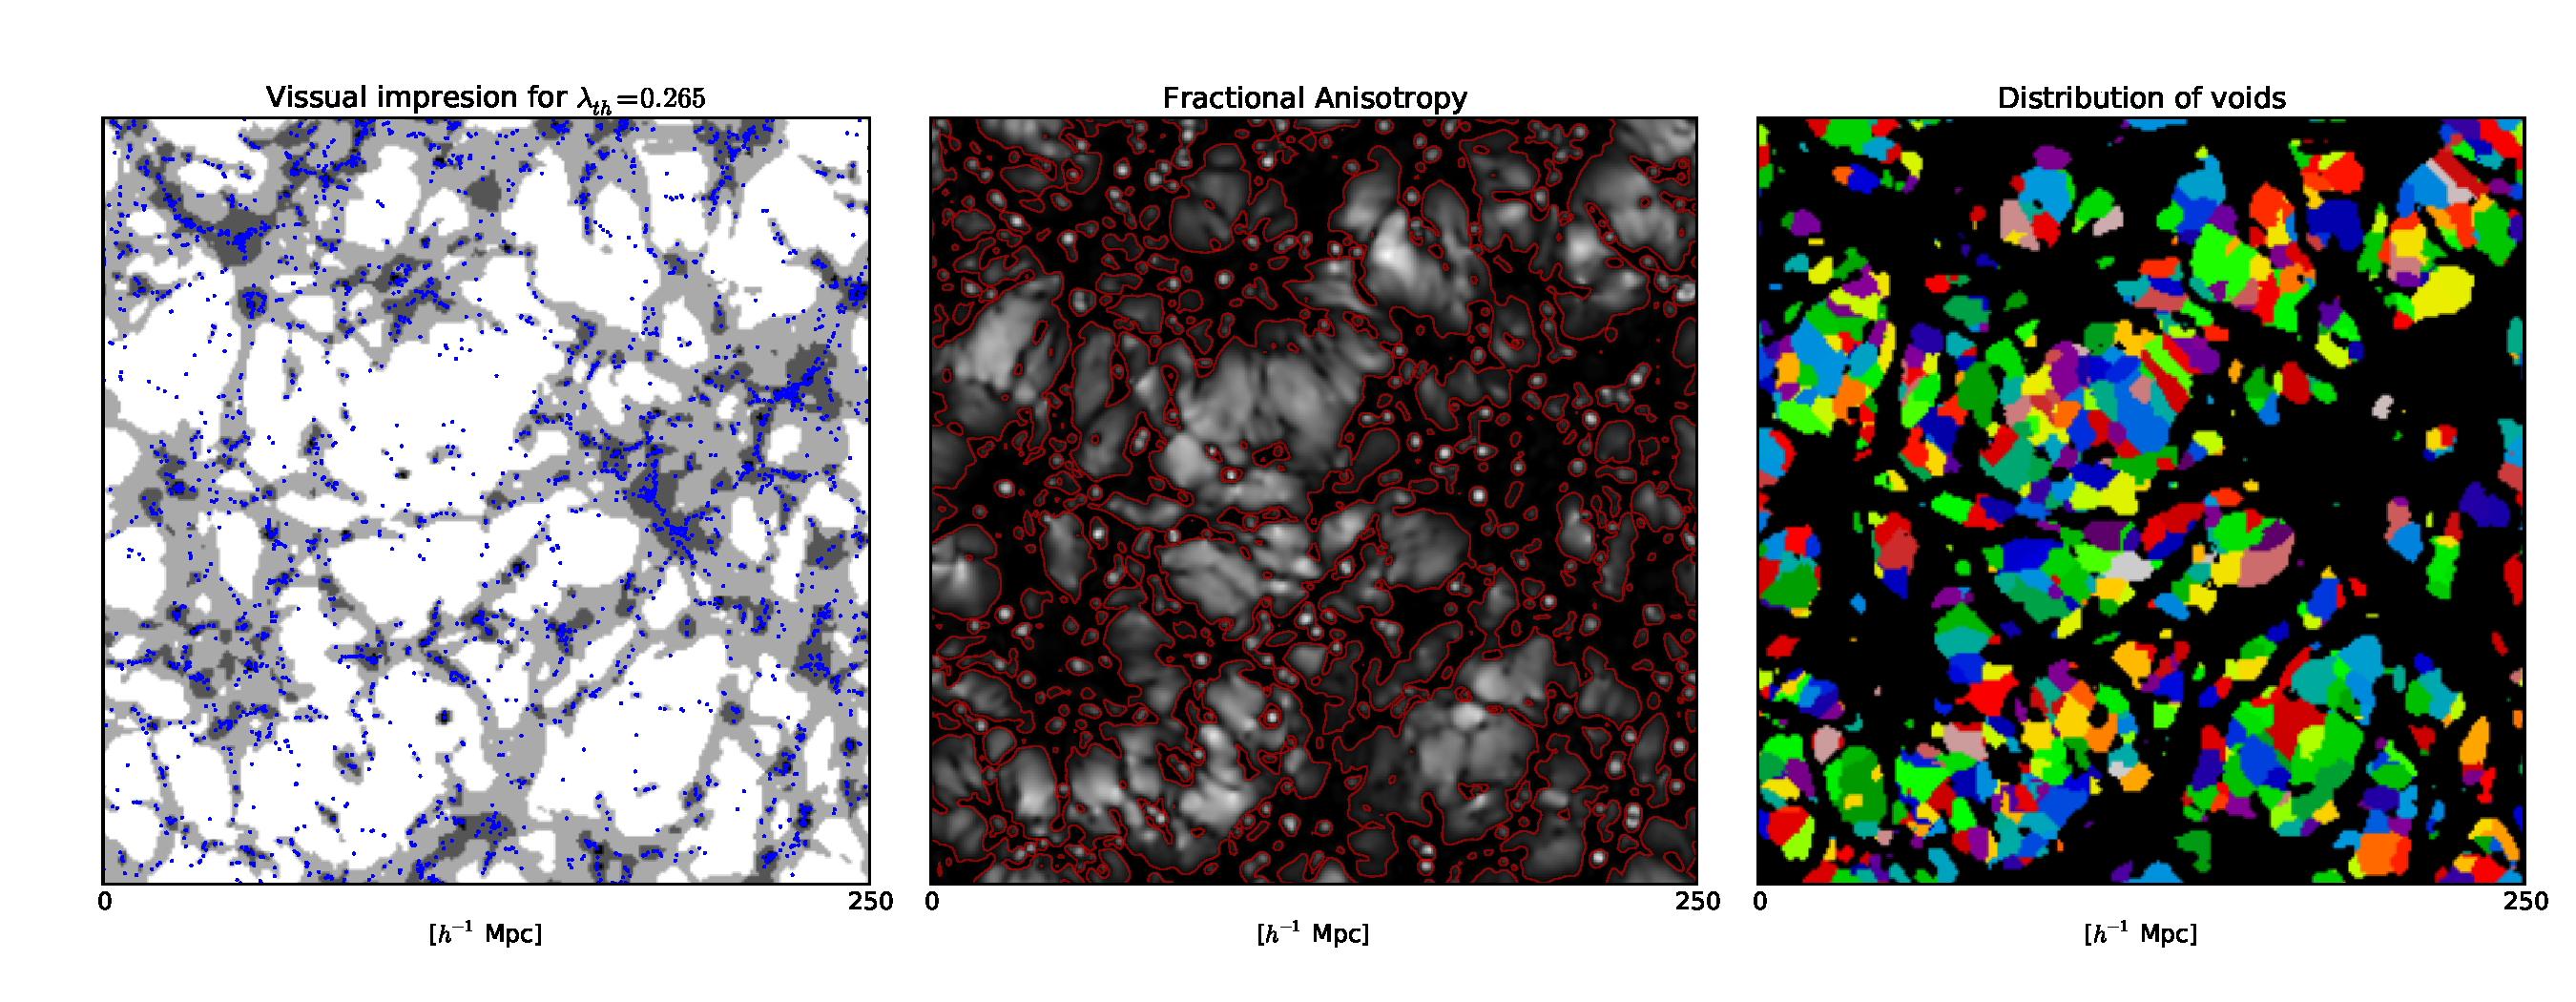
\includegraphics[trim = 16mm 8mm 5mm 12mm, clip, keepaspectratio=true,
  width=0.73\textheight]{./figures/cosmicweb_FA_Tweb.pdf}
  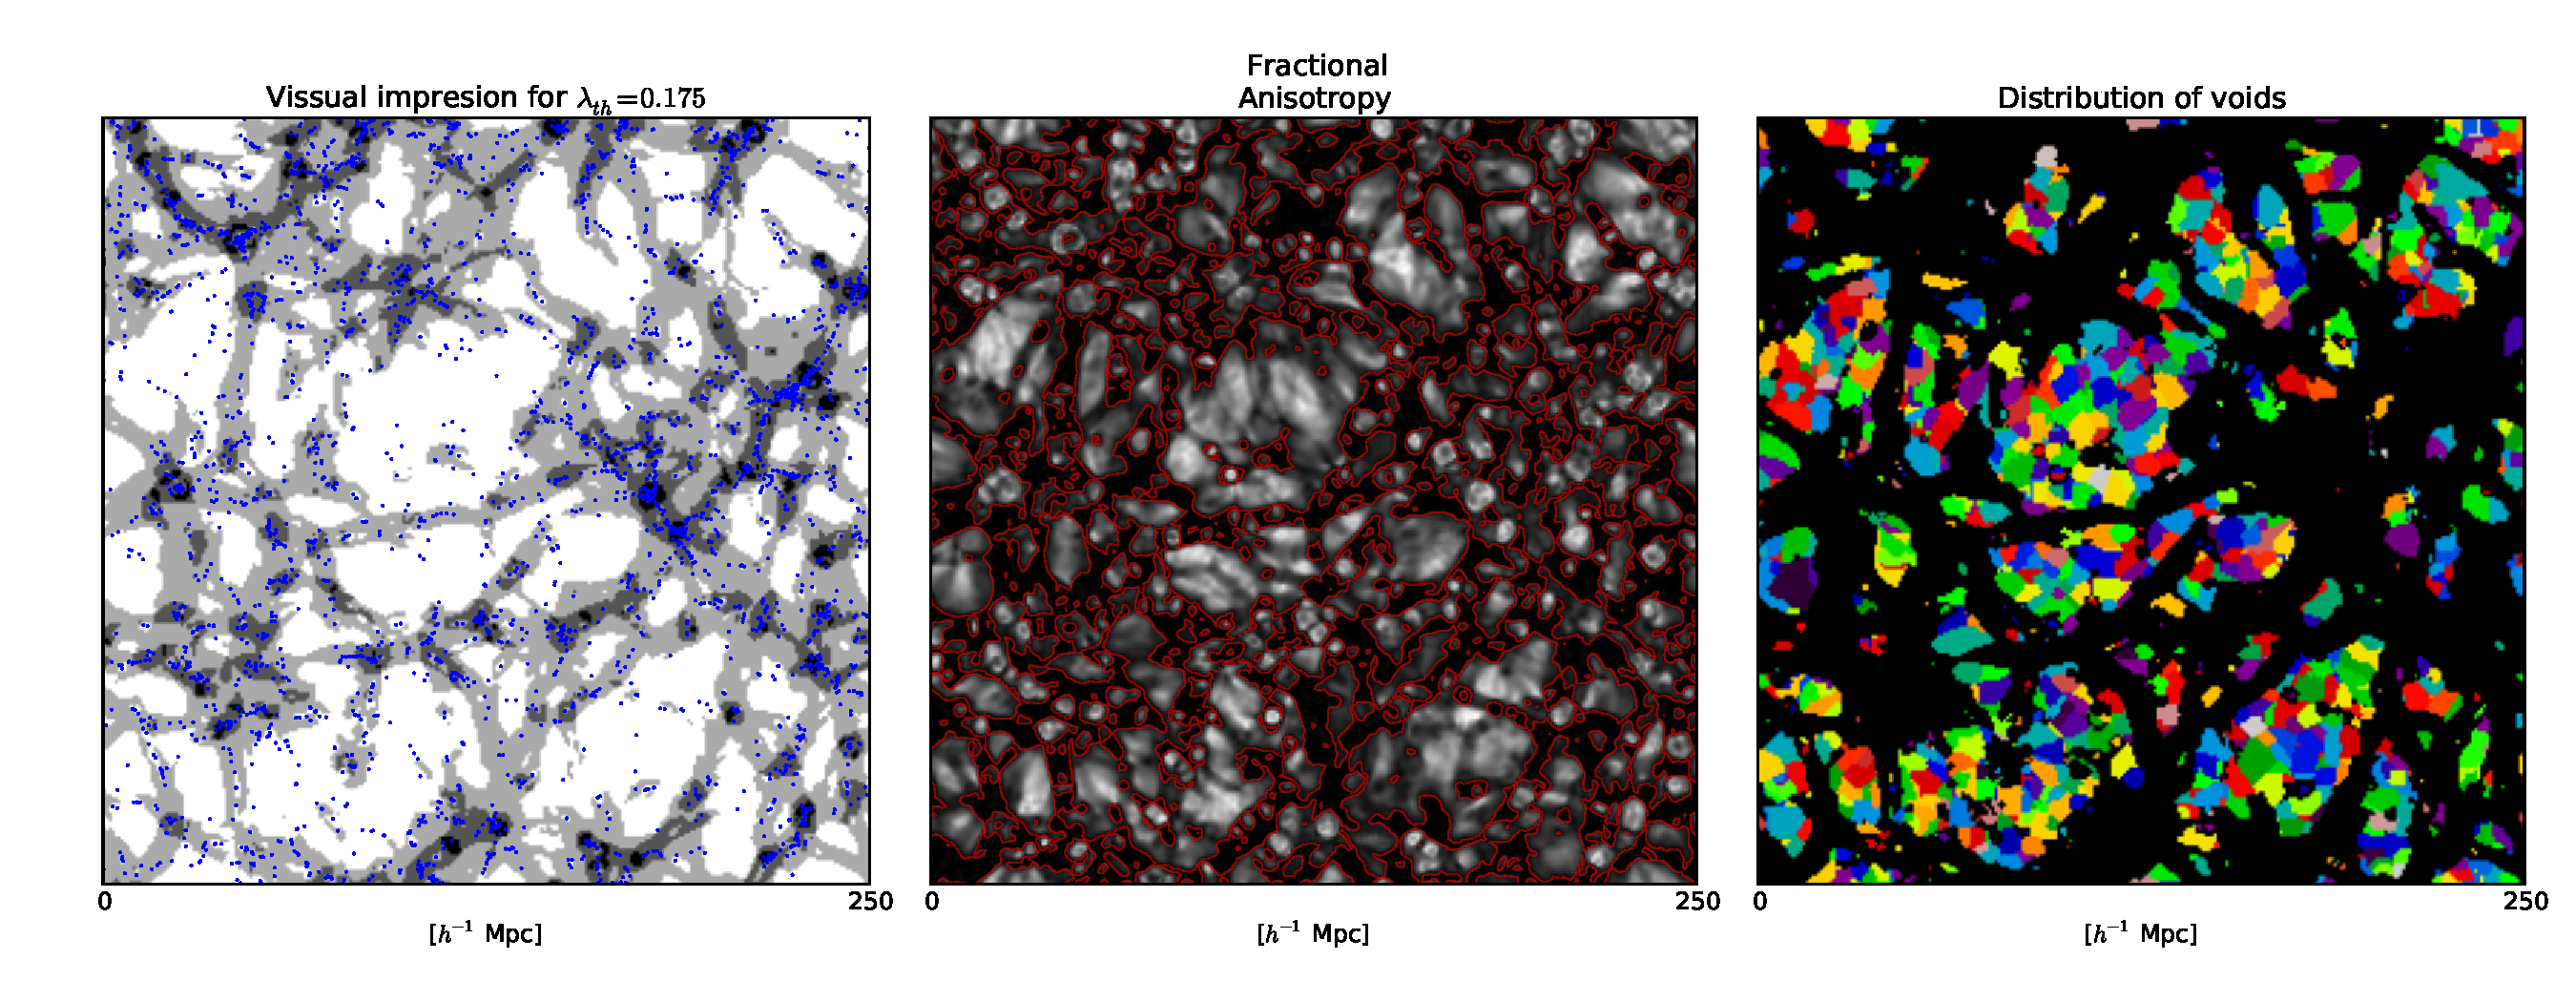
\includegraphics[trim = 16mm 8mm 5mm 12mm, clip, keepaspectratio=true,
  width=0.73\textheight]{./figures/cosmicweb_FA_Vweb.pdf}
  \caption{Left colum. Visual impression of the 
  FA field over a slide of the simulation for each web scheme (T-web, upper 
  panels. V-web, middle panels). 
  Middle column. Components of the Cosmic Web using $\lambda_{th}$
  values that put an upper bound of $FA=0.95$ to voids. Voids
  corresponds with white, sheets to gray, filaments to dark gray and
  knots with black regions. 
  Right column. Sketches the distribution of the catalogued voids by
  our method.}
  \label{fig:FA_field}
\end{figure*}
%.........................................................................


%-------------------------------------------------------------------------
\subsection{Fractional anisotropy as a void tracer}
\label{subsec:web_voids}
%-------------------------------------------------------------------------


%-------------------------------------------------------------------------
%FIGURE 2: Distributions of FA and density regarding the Lambda_1 eigenvalue
\begin{figure*}
\centering

  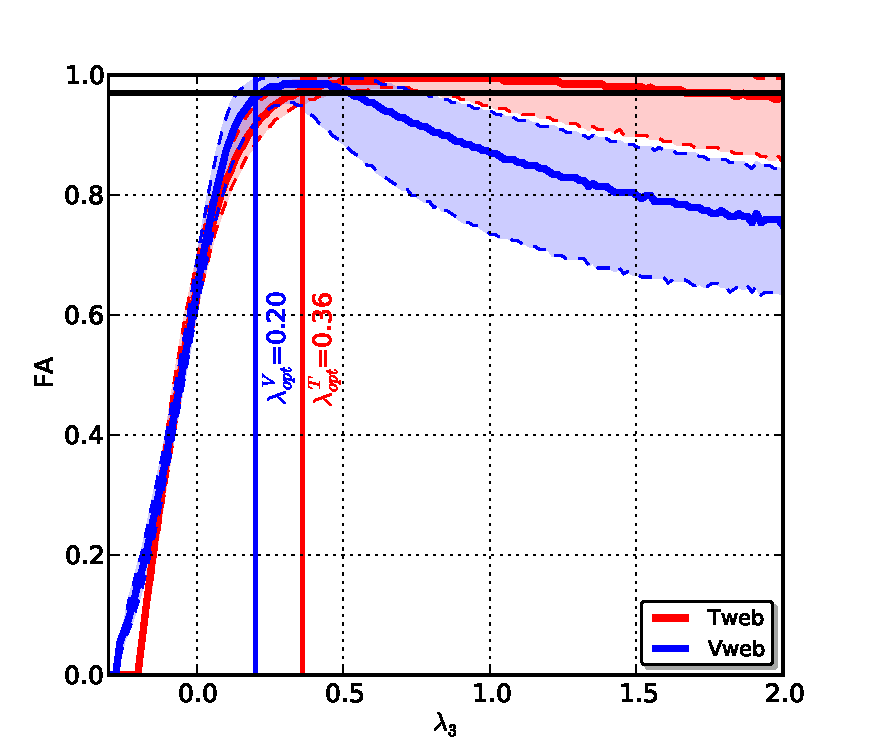
\includegraphics[trim = 2mm 2mm 5mm 10mm, clip, keepaspectratio=true,
  width=0.3\textheight]{./figures/FA_L1.pdf}
  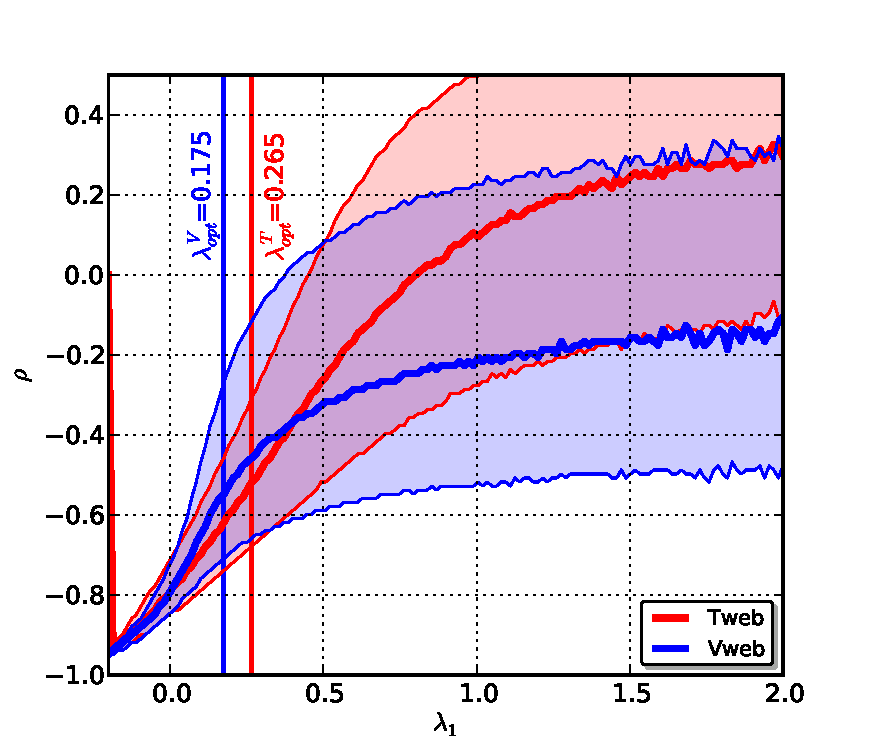
\includegraphics[trim = 2mm 2mm 5mm 10mm, clip, keepaspectratio=true,
  width=0.3\textheight]{./figures/delta_L1.pdf}  
  
  \captionof{figure}{\small Distributions of the FA (left panel) and the 
  density field (right panel) with respect to the eigenvalue $\lambda_1$ 
  for each web scheme (Tweb, red lines. Vweb, blue lines) as calculated 
  over all cells of the grid. Thick central lines correspond with the median 
  and filled regions with the $50\%$ of the distribution.}

  \label{fig:L1_correlations}

\end{figure*}
%.........................................................................


Voids are regions where $\lambda_3\leq\lambda_2\leq
\lambda_1\leq\lambda_{th}$. 
This implies that a void is completely fixed by the relative strength
of the $\lambda_1$ eigenvalue with respect to the $\lambda_{th}$.   
As we  increase/decrease the threshold value $\lambda_{th}$, voids
increase/decrease progressively through contours of
increasing/decreasing $\lambda_1$.   
 
Voids are thus characterized by low values of both FA and
$\lambda_1$. 
In Fig. \ref{fig:L1_correlations} we show that the these two values
are indeed closely correlated.  
The left panel shows the correlation between $\lambda_1$ and $FA$ for
all the grid cells in the simulation while the right panel shows the
correlation between $\lambda_1$ and the local overdensity $\delta$.  
This shows that the overdensity has a large scatter at fixed
$\lambda_1$. 

From Figs. \ref{fig:FA_field} and \ref{fig:L1_correlations} we
conclude that the FA is a good tracer of voids as it is almost perfectly
correlated with low values of $\lambda_1$. 
We propose that voids should be composed completely by regions of
FA$<0.95$.
If we increase the values of $\lambda_1$ from its minimum until it
we reach FA$=0.95$ in \ref{fig:L1_correlations} we find that this
correspond to critical values of $\lambda_{1}^T = 0.265$ and
$\lambda_{1}^V = 0.175$ for the Tweb and Vweb, respectively.
This means that setting $\lambda_{th}$ to either
$\lambda_{1}^T$/$\lambda_{1}^{V}$ automatically produces voids with
all the cells $FA<0.95$.   
The middle column in Fig. \ref{fig:FA_field} shows the web
classification for this choice of $\lambda_{th}$, demonstrating that
it is a sensible choice to define voids. 

   
%-------------------------------------------------------------------------
\subsection{Defining voids with a watershed algorithm}
\label{sec:watershed}
%-------------------------------------------------------------------------


Once established the FA as a good tracer of voids, the next step is to
find individuals voids in the overall distribution. For this purpose, we
use the \textit{watershed transform algorithm} \citep{Beucher79,Beucher93}, 
in which a void is identified as the catching basin of a local minimum of
the FA. The use of this algorithm is advantageous as it is parameter-free 
and does not require any assumption on the shape and morphology of voids. 


Previous implementations of this technique as those of \citet{Platen07,
Neyrinck08} have shown remarkable results regarding voids finding, however
they use the density field instead of the FA field. On the other hand, we 
use a \textit{cloud-in-cell} (\texttt{CIC}) algorithm on a Cartesian mesh for 
estimating the density and tensor fields, instead of the more sophisticated 
\textit{Delaunay tessellation for field estimator} (\texttt{DTFE}) technique 
\citep{Schaap00}, but our implementation of the watershed transform should 
not be significantly affected as we are interested in low density regions 
where the \texttt{CIC} gives similar estimations.


As suggested by \citet{Platen07} and references therein, it is necessary to
apply a threshold merger in order to reduce spurious features and to avoid 
void hierarchization. A natural choice is a threshold of $\delta = -0.8$, 
which means that any ridge between two voids with density below that value
would be removed and the respective voids merged. As we are working with the
FA, the equivalent threshold according to Fig. \ref{fig:L1_correlations} is
$FA = 0.65$. In right panels of Fig. \ref{fig:FA_field} we show the resulting
catalogues of voids for both schemes.


%Once set the optimal thresholds for the web schemes, we proceed in Fig. 
%\ref{fig:FAShapeness} to sample the FA and the prolateness for a random 
%sample of cells previously classified into one of the four
%environments.
 
%The prolateness is introduced here for differentiating sheets and filaments
%featuring high FA values. 
%In order to illustrate the underlying local 
%dynamics sampled by the cells, we also sketch different spheroidal 
%geometries according to the relative strength of each eigenvalue, and 
%then, we associate them to different ranges of the FA and the prolateness. 

%From this, we conclude sheets display very anisotropic distributions, 
%namely above $FA=0.95$. They are also biased towards oblate geometries, 
%however there are some elongated sheets as well. Filaments are not as 
%anisotropic as sheets, ranging from middle up to high FA values. They 
%exhibit prolate geometries, but a considerable fraction of them are biased 
%towards slightly more oblate values. Voids and knots are the only 
%environments featuring with low FA values, thus indicating very isotropic 
%expanding/collapsing dynamics at their centres. However, voids span over 
%a very wide range of FA and geometries, whereas knots only span over low 
%to middle FA values and display a biased oblate geometry.



%*************************************************************************
\section{Results}
\label{sec:results}
%*************************************************************************


%-------------------------------------------------------------------------
\subsection{Enclosed mass}
\label{subsec:enclosedmass}
%-------------------------------------------------------------------------


When we analyse individual density profiles of voids (see left panels of
Fig. \ref{fig:RhoVel}), they seem to be distributed in two different 
families, differentiated by the presence or absence of a compensation 
ridge (e.g. see also Fig. 14 of \citet{Colberg05}). In order to 
discriminate each void in one of the families, we propose the compensation 
index $\mathcal{C}$, which is defined as the mass of a void enclosed in a 
spherical volume of radius $R$ and normalized by the mass of the same 
volume as assuming the mean background density instead

\eq{compensation}
{\mathcal{C} = \frac{M_v}{\overline{M}} = \frac{3}{2R^{3}} \int_0^{R} [\delta(r) + 1] r^2 dr}

We choose an integration radius of $R=4r_{eff}$, that is large enough to 
enclose the compensation ridge for a typical void in case there is one. 
This leads us to voids with $\mathcal{C}>1$ having more mass than expected, 
constituting the family of overcompensated voids. These voids generally 
exhibit a compensation ridge associated to dense nearby structures. In the 
same fashion, voids with $\mathcal{C}<1$ constitute the family of 
subcompensated voids.


%-------------------------------------------------------------------------
\subsection{The void size distribution}
\label{subsec:shape_voids}
%-------------------------------------------------------------------------


%.........................................................................
%FIGURE 3: volume functions
\begin{figure}
\centering

  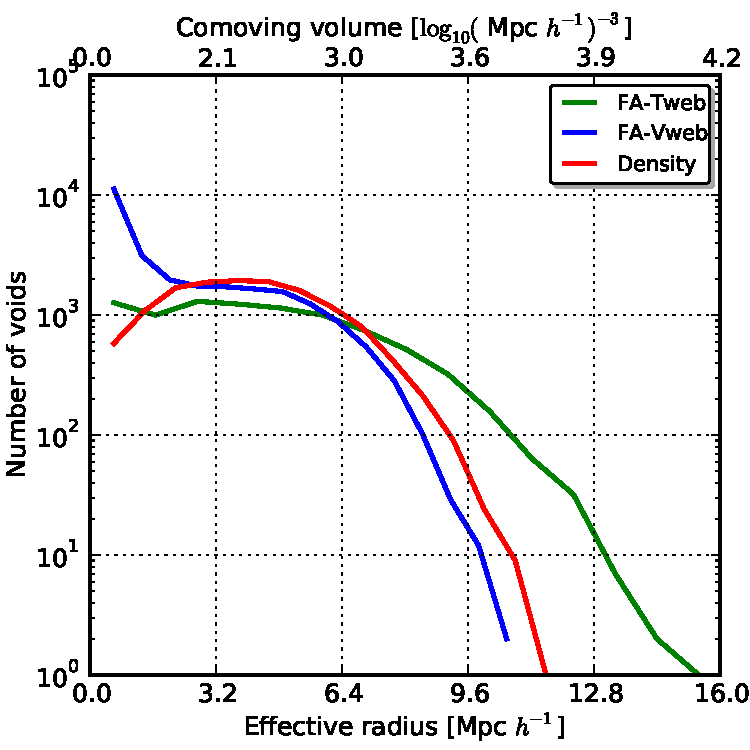
\includegraphics[trim = 0mm 0mm 0mm 0mm, clip, keepaspectratio=true,
  width=0.3\textheight]{./figures/voids_regions_volume_all.pdf}

  \captionof{figure}{\small Volume size distribution of voids for both
  catalogues. FA-Tweb (red curves), FA-Vweb (blue curves).
  Continuous lines corresponds with the total number of voids, dot-dashed
  with sub-compensated voids and dashed lines with over-compensated voids. }

  \label{fig:volume_function}

\end{figure}
%.........................................................................


Since the shape of the voids exhibit a wide range of geometries, a common 
way to represent their size is through the equivalent spherical radius or
effective radius, defined as $r_{eff} = [3/(4\pi)V]^{1/3}$, with $V$ the 
total volume of the void. As mentioned before, we applied a threshold merger
in order to avoid void hierarchization, what means we are working with the
top hierarchy of voids. We limit our findings to voids with effective radius
greater than the smoothing length of the density field, i.e. $\sim 1$\hMpc. 
Below that scale numerical resolution effects becomes important. We find a
volume filling fraction of voids of $54.88\%$ of the total volume of the 
simulation for the FA-Tweb and $47.06\%$ for the FA-Vweb.


In Fig. \ref{fig:volume_function} we show the void size distributions
for both schemes and for the overall distribution of voids as well as for 
overcompensated and subcompensated void subsamples. The central region of
the distributions ($3$\hMpc\ -- $6$\hMpc), exhibit an approximately flat 
shape, contrary to expected from highly non-linear structures like dark 
matter halos, where the abundances increase for smaller structures. 
The distribution of the FA-Tweb is consistent with a two-barrier problem 
\citep{Sheth04}: formation of large voids is inhibited by the 
\textit{void-in-void} problem (first barrier), where large voids are 
constituted hierarchically of smaller ones. In turn, formation of small 
voids is damped by the \textit{void-in-cloud} problem (second barrier), 
where nearby collapsing structures limit the abundance of embedded small 
voids.


The FA-Vweb scheme does not tackle properly the \textit{void-in-cloud} 
problem as it predicts large abundances of smaller voids. However, an 
interesting result is the difference between the overcompensated and 
subcompensated subsamples. Subcompensated voids, which are expected to 
be embedded in low-density regions like walls and larger voids, exhibit
smaller abundances compatible with the result of the FA-Tweb. Then, the 
most dramatic contribution to the overabundance of small voids for the 
FA-Vweb comes from overcompensated voids. This implies that, although
nearby non-linear structures squeeze out embedded smaller voids, the
rapid and isotropic collapse in these zones, along with the more rugged 
nature of the velocity field make these voids still detectable by this 
scheme.


For both schemes overcompensated voids are more abundant, however at 
larger scales abundances of subcompensated voids become comparable. This 
is somehow expected as larger voids are more likely to abut other voids.
A recent estimation of the radius of the local void gives $r_{LV}\approx
10$ Mpc \citep{Nasonova11}. Taking the dimensionless Hubble constant as 
$h = 0.70$, the size of the local void would be around $r_{eff} = 7$
\hMpc\ in the shown distribution. For both schemes, this places the local
void as a rather common void in terms of size, and more likely to be
overcompensated.


%-------------------------------------------------------------------------
\subsection{Physical profiles of voids}
\label{subsec:properties_voids}
%-------------------------------------------------------------------------


%.........................................................................
%FIGURE 4: Density profile of voids for each defined scheme
\begin{figure*}
\centering
  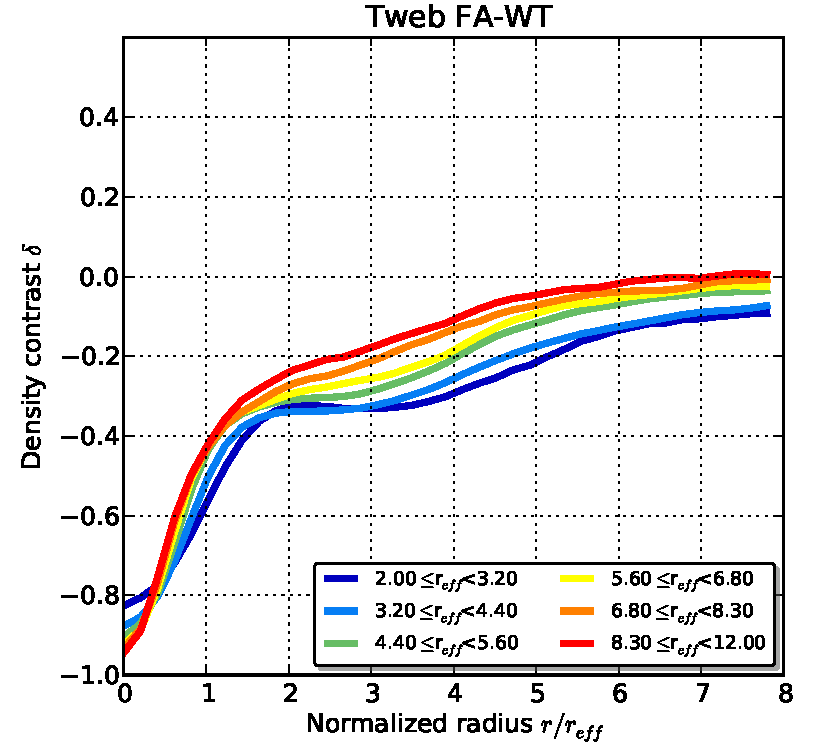
\includegraphics[trim = 1mm 0mm 5mm 0mm, clip, keepaspectratio=true,
  width=0.24\textheight]{./figures/voids_density_TwebFAG0.pdf}
  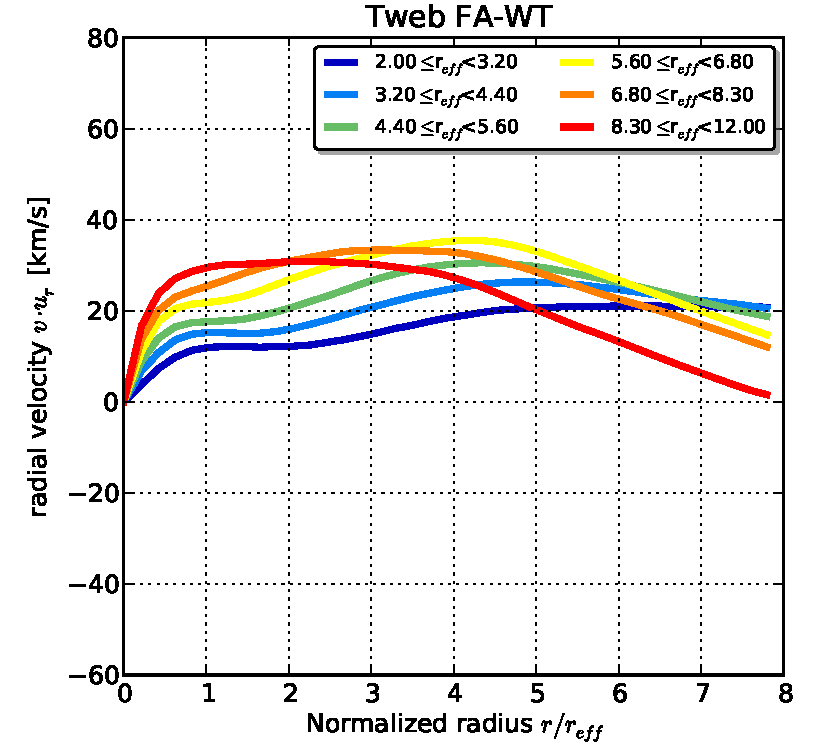
\includegraphics[trim = 1mm 0mm 5mm 0mm, clip, keepaspectratio=true,
  width=0.24\textheight]{./figures/voids_velocity_TwebFAG0.pdf}
  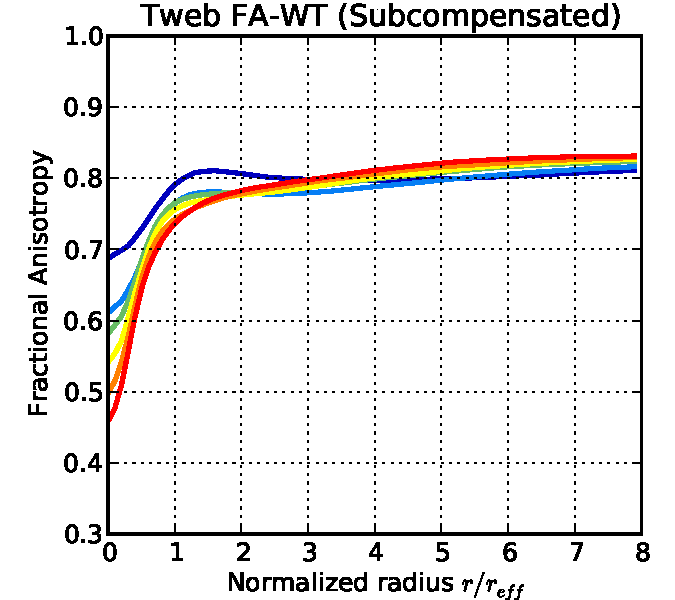
\includegraphics[trim = 1mm 0mm 5mm 0mm, clip, keepaspectratio=true,
  width=0.24\textheight]{./figures/voids_FA_TwebFAG0.pdf}
  
  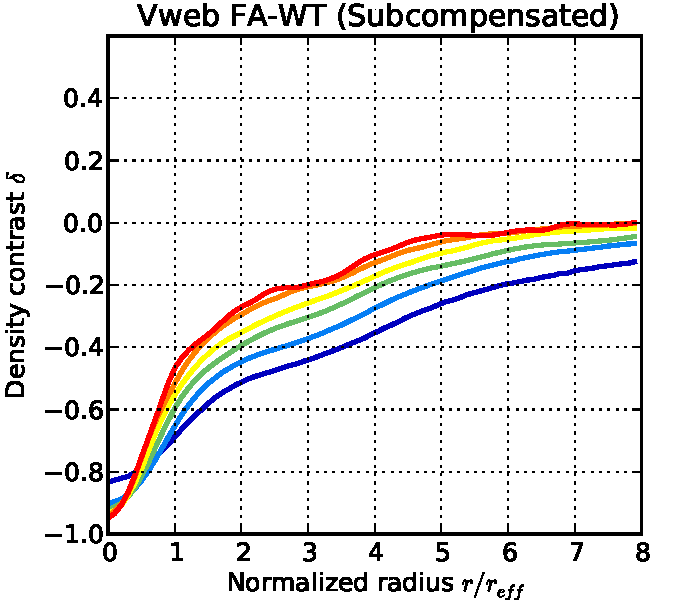
\includegraphics[trim = 1mm 0mm 5mm 0mm, clip, keepaspectratio=true,
  width=0.24\textheight]{./figures/voids_density_VwebFAG0.pdf}
  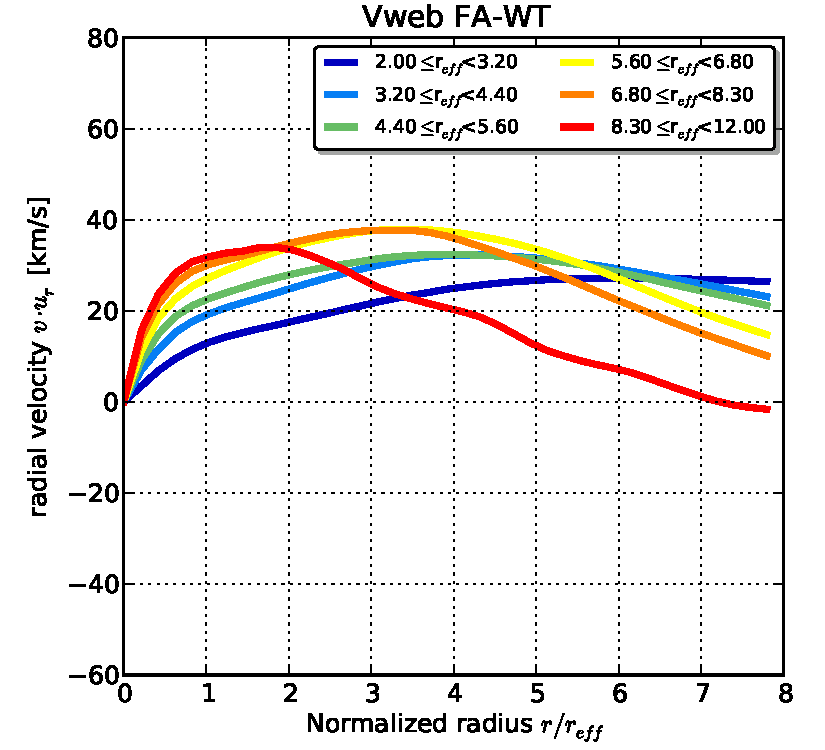
\includegraphics[trim = 1mm 0mm 5mm 0mm, clip, keepaspectratio=true,
  width=0.24\textheight]{./figures/voids_velocity_VwebFAG0.pdf}
  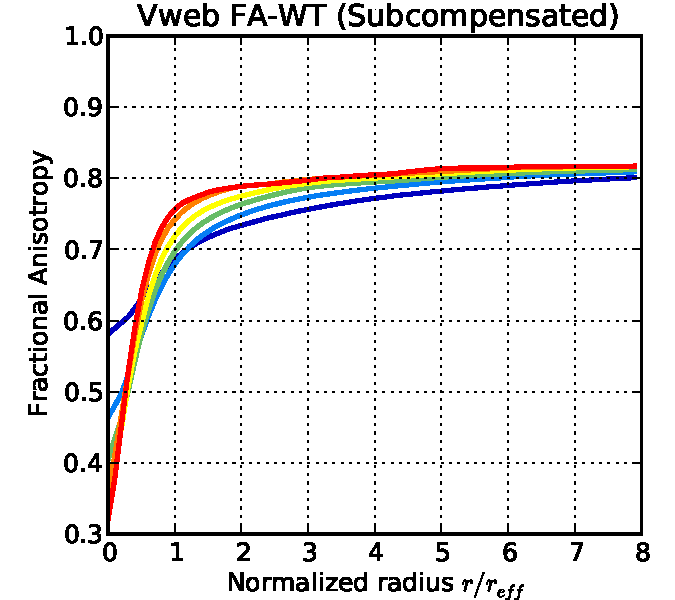
\includegraphics[trim = 1mm 0mm 5mm 0mm, clip, keepaspectratio=true,
  width=0.24\textheight]{./figures/voids_FA_VwebFAG0.pdf}
  
  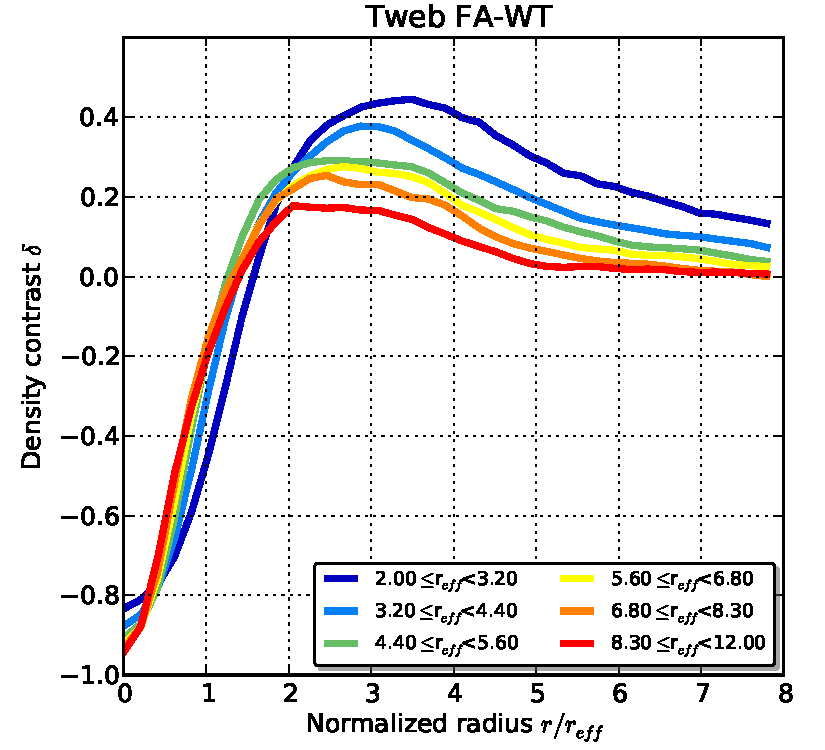
\includegraphics[trim = 1mm 0mm 5mm 0mm, clip, keepaspectratio=true,
  width=0.24\textheight]{./figures/voids_density_TwebFAG1.pdf}
  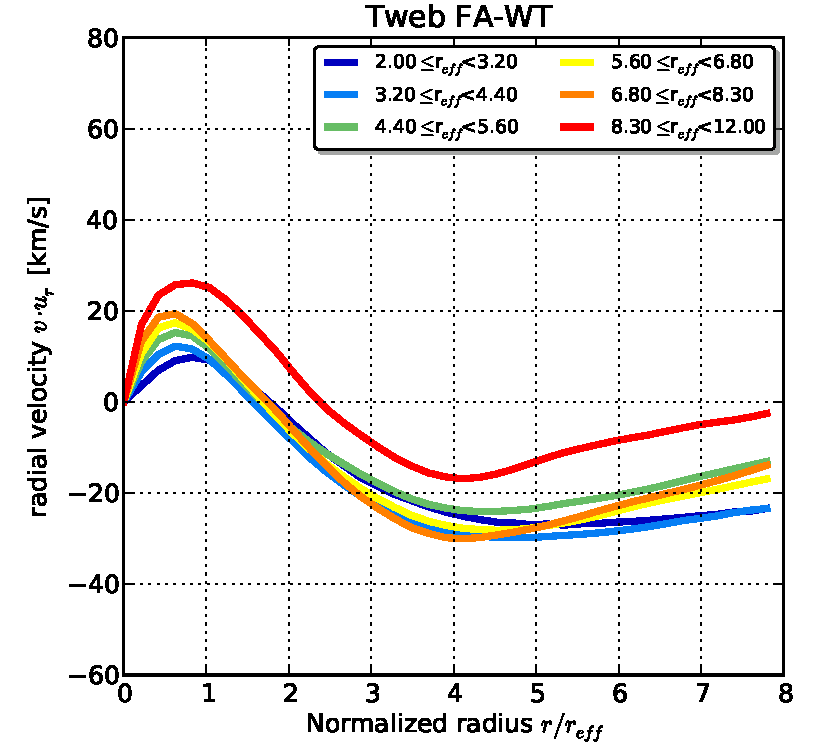
\includegraphics[trim = 1mm 0mm 5mm 0mm, clip, keepaspectratio=true,
  width=0.24\textheight]{./figures/voids_velocity_TwebFAG1.pdf}
  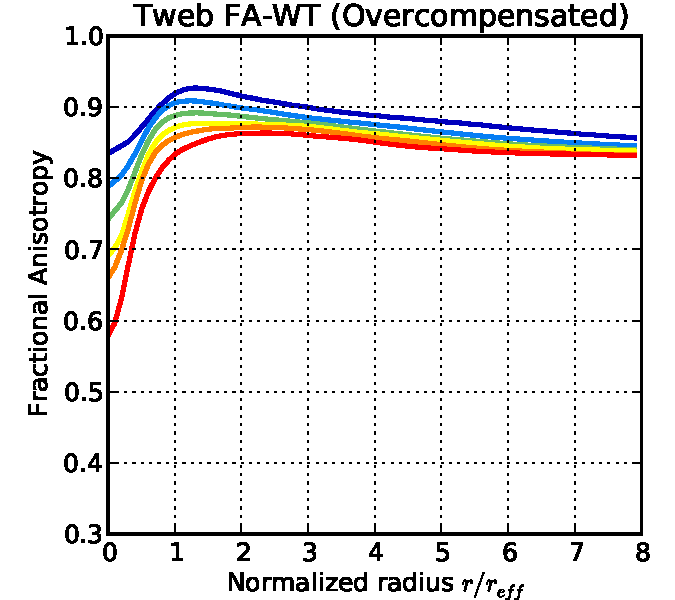
\includegraphics[trim = 1mm 0mm 5mm 0mm, clip, keepaspectratio=true,
  width=0.24\textheight]{./figures/voids_FA_TwebFAG1.pdf}

  
  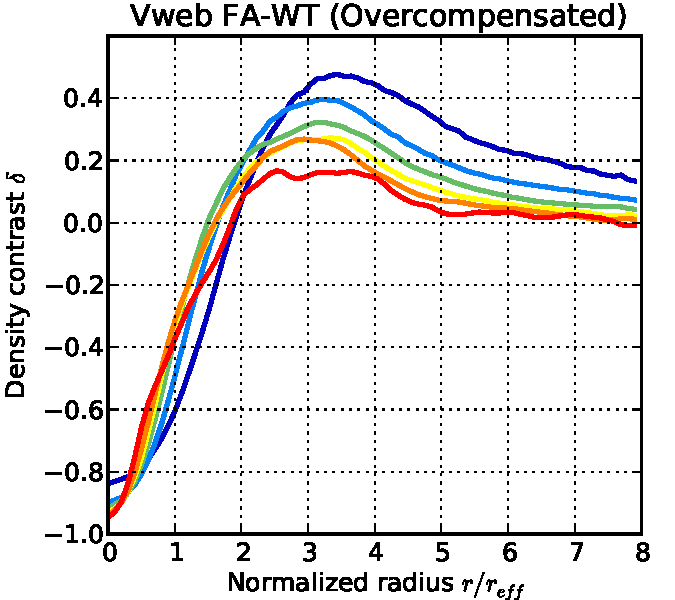
\includegraphics[trim = 1mm 0mm 5mm 0mm, clip, keepaspectratio=true,
  width=0.24\textheight]{./figures/voids_density_VwebFAG1.pdf}
  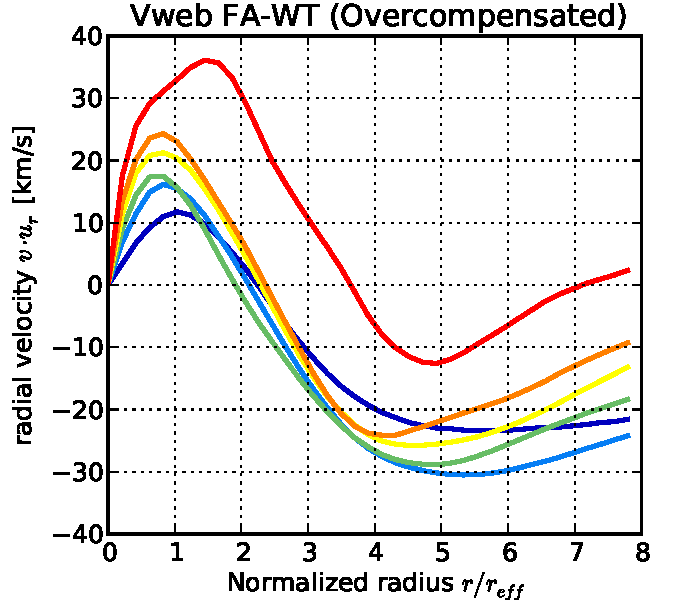
\includegraphics[trim = 1mm 0mm 5mm 0mm, clip, keepaspectratio=true,
  width=0.24\textheight]{./figures/voids_velocity_VwebFAG1.pdf}
  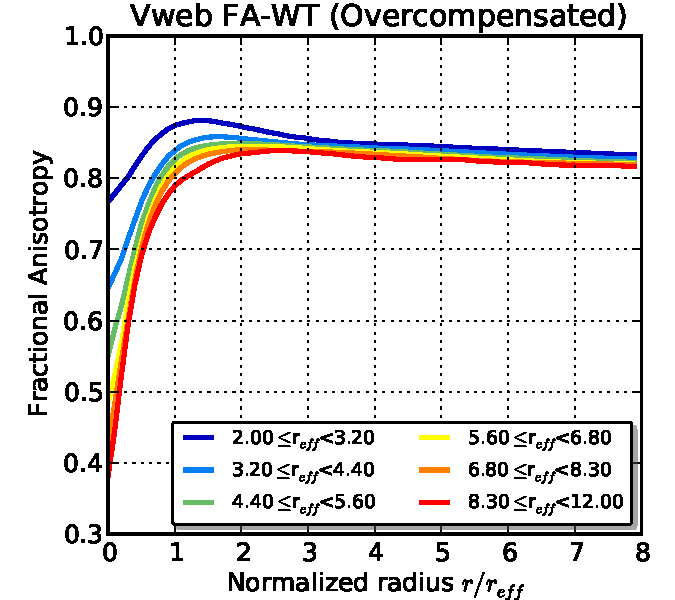
\includegraphics[trim = 1mm 0mm 5mm 0mm, clip, keepaspectratio=true,
  width=0.24\textheight]{./figures/voids_FA_VwebFAG1.pdf}  
  

  \captionof{figure}{\small Physical internal properties of voids for 
  the two finding scheme. Density field (left panels), radial-projected
  velocity field (middle panels) and FA field (right panels). The analysis
  is performed for both, subcompensated (first two rows) and overcompensated
  voids (last two rows).}

  \label{fig:RhoVel}
  \vspace{0.1 cm}

\end{figure*}
%.........................................................................


In Fig. \ref{fig:RhoVel} we analyse the internal properties of the found 
voids. We calculate the contrast density, radial-projected velocity and 
FA profiles. For this purpose we catalogue all the voids into several 
radial bins in order to capture possible size effects. Then, for each void, 
we take the distance of each member cell to the void centre along with the 
properties of interest. Normalizing these distances with the effective 
radius, we stack all the voids catalogued in a radial bin in order to 
compute radial profiles of the properties of interest.


%.........................................................................
\subsubsection{Density profiles}
\label{subsubsec:density_voids}
%.........................................................................


In Fig. \ref{fig:RhoVel} we analyse the internal properties of the found 
voids. We calculate the contrast density, radial-projected velocity and 
FA profiles. For this purpose we catalogue all the voids into several 
radial bins in order to capture possible size effects. Then, for each void, 
we take the distance of each member cell to the void centre along with the 
properties of interest. Normalizing these distances with the effective 
radius, we stack all the voids catalogued in a radial bin in order to 
compute radial profiles of the properties of interest.

%.........................................................................
\subsubsection{Velocity profiles}
\label{subsubsec:velocity_voids}
%.........................................................................

%.........................................................................
\subsubsection{FA profiles}
\label{subsubsec:FA_voids}
%.........................................................................


%*************************************************************************
\section{Conclusions}
\label{sec:conclusions}
%*************************************************************************


%*************************************************************************
\section*{Acknowledgments}  
%*************************************************************************


\bibliographystyle{latex/mn2e}
\bibliography{references}


%.........................................................................
%FIGURE -: FA of some regions and shape illustration
%\begin{flushleft}
%\begin{figure*}
%\centering
%  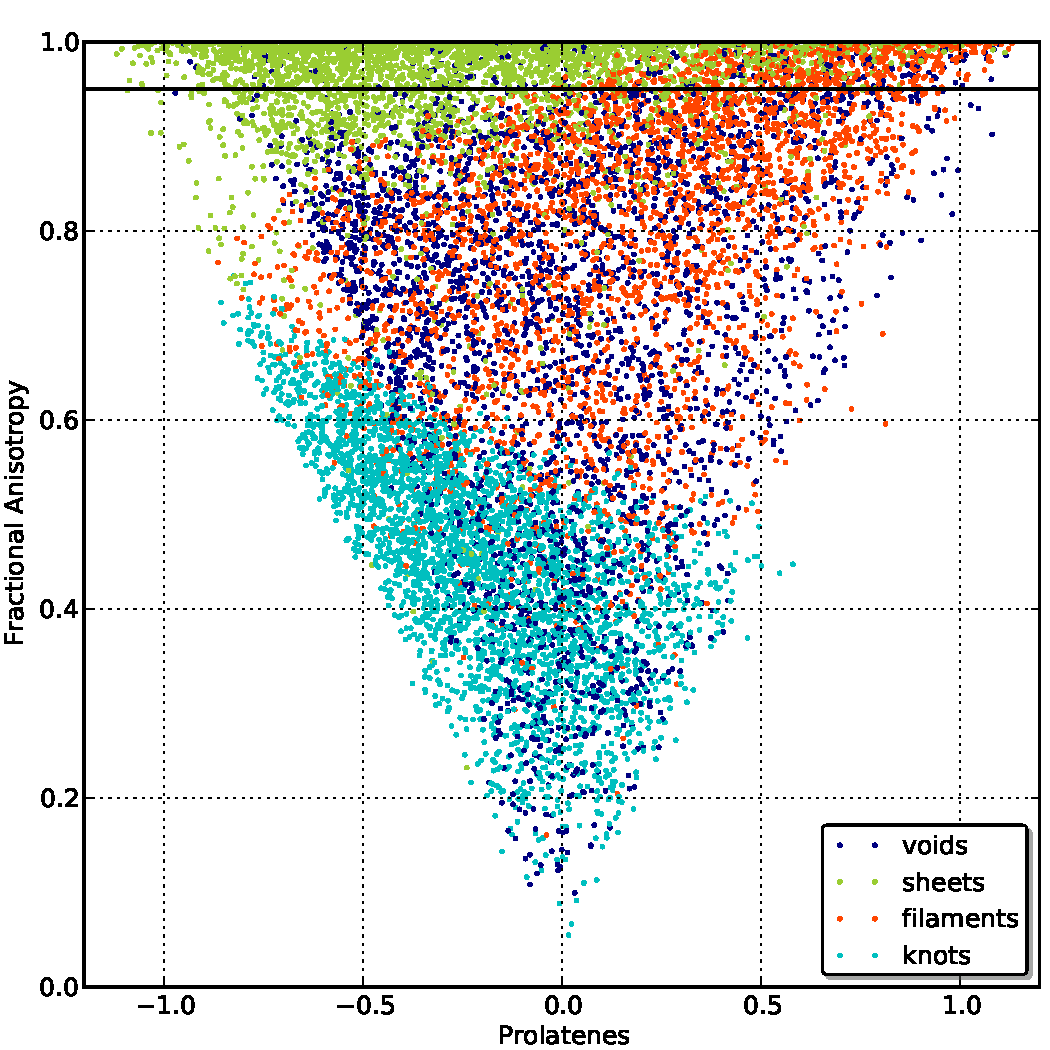
\includegraphics[trim = 0mm 1mm 0mm 1mm, clip, keepaspectratio=true,
%  width=0.3\textheight]{./figures/FA_Prolatenes_Vweb.pdf}
%  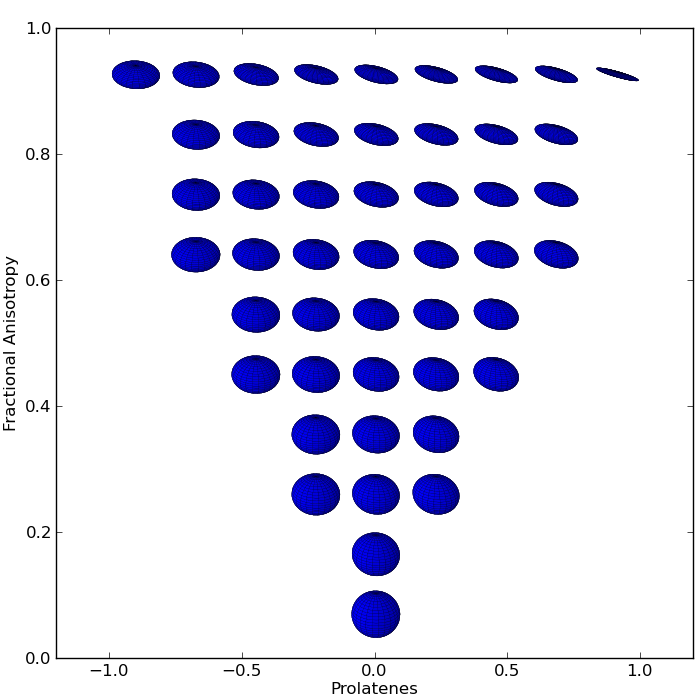
\includegraphics[trim = 0mm 1mm 0mm 1mm, clip, keepaspectratio=true,
%  width=0.3\textheight]{./figures/FA_Prolatenes.png}  
  
%  \captionof{figure}{\small Fractional anisotropy and prolateness for a 
%  random sample of cells (left panel) and for different spherical 
%  geometries (right panel). For the cells, each environment is coded with
%  a different colour, i.e. voids corresponds with dark blue points, 
%  sheets with green, filaments with orange and knots with cyan. The axis 
%  of the spheroids are computed from the relative strengths of the 
%  eigenvalues, so their shape sketch the relative expanding/collapsing 
%  dynamics into each direction.}

%  \label{fig:FAShapeness}
%  \vspace{0.1 cm}

%\end{figure*}
%\end{flushleft}
%.........................................................................
\end{document}
